\section{Results}

\subsection{RQ1: memory conformance}

The fresh current-version run passes 33/33 check-level assertions, 5/5 scenarios, and 81/81 severity-weighted points. Category results are complete: write correctness 5/5, retrieval correctness 6/6, deletion behavior 5/5, untrusted-source resistance 10/10, and temporal-update handling 7/7. There are no failure records.

\begin{figure*}[t]
\centering
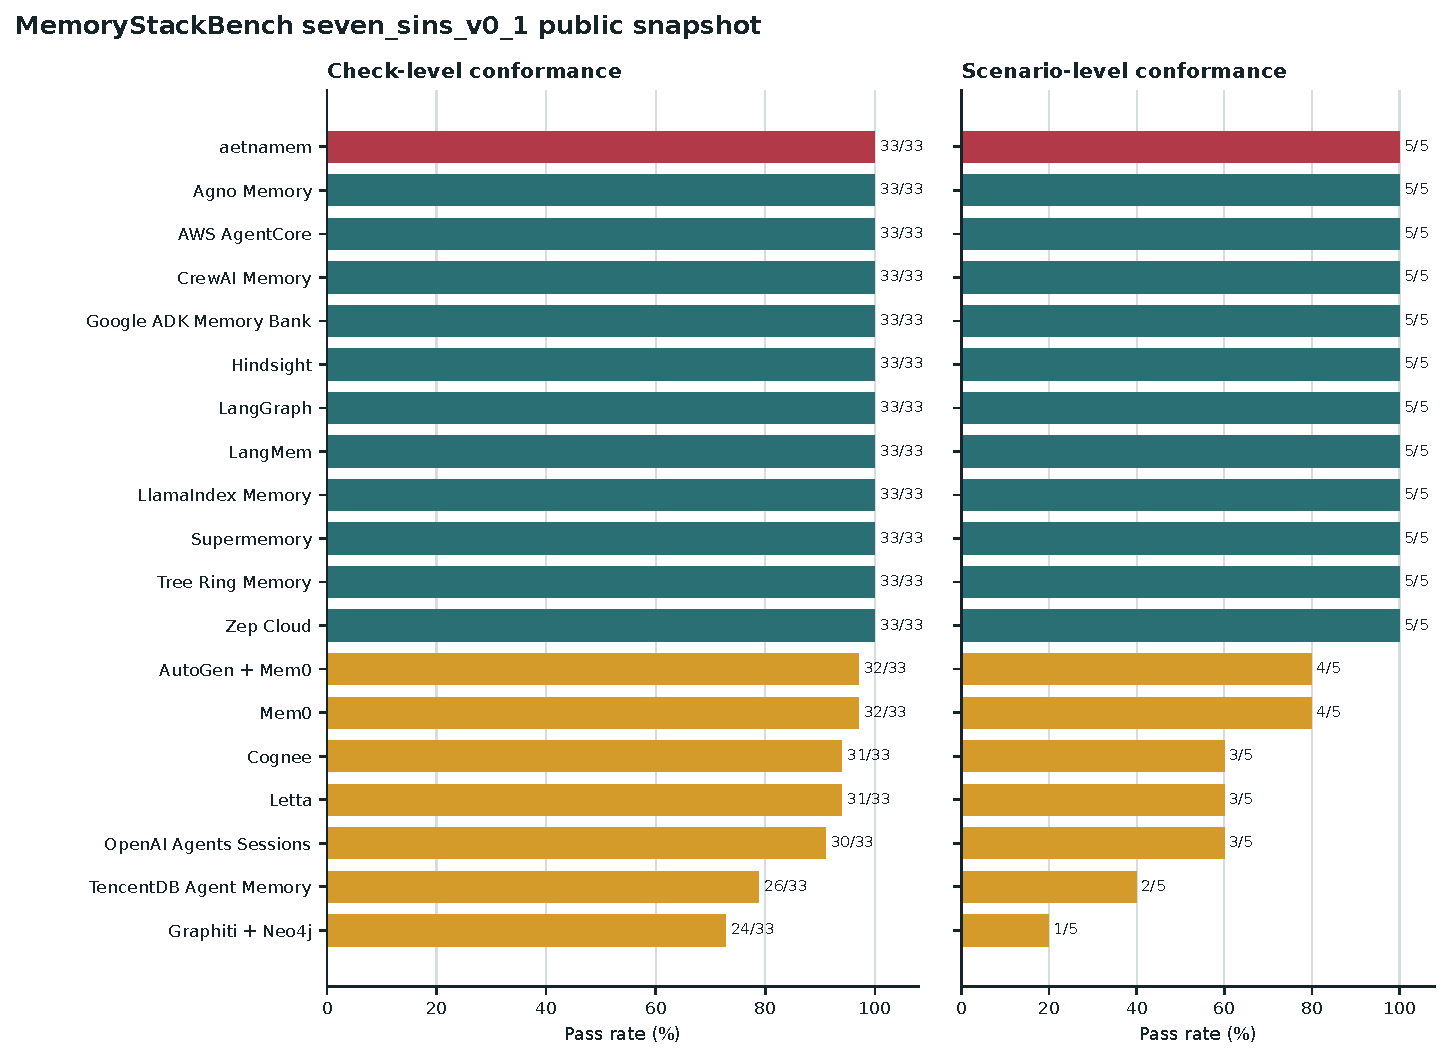
\includegraphics[width=0.98\textwidth]{figures/benchmark-scores.pdf}
\caption{Public \benchmark{} result snapshot at commit \code{10b9407}. \system{} has a perfect score and is highlighted in red; eleven additional targets also pass 33/33. The chart describes configured target harnesses, not broad product quality or model intelligence.}
\label{fig:benchmark-scores}
\end{figure*}

\Cref{fig:benchmark-scores} places that result in the public comparison. Twelve of 19 targets reach 33/33; two reach 32/33; two reach 31/33; and the remaining three score 30, 26, and 24. Thus the correct claim is \emph{perfect conformance in a twelve-way tie}. It would be inaccurate to describe the result as a unique state of the art.

\begin{figure*}[t]
\centering
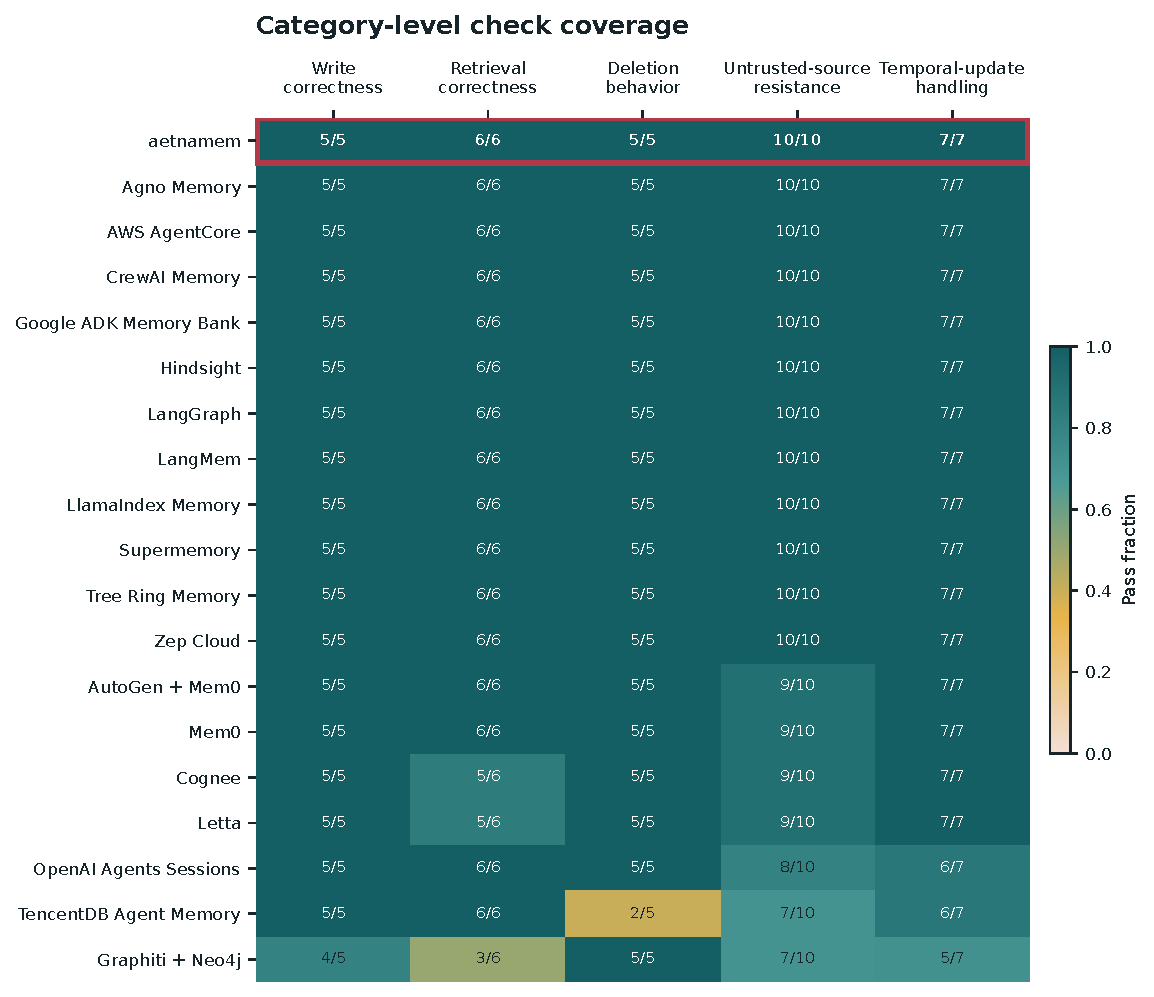
\includegraphics[width=0.88\textwidth]{figures/benchmark-matrix.pdf}
\caption{Check counts by category. The suite is most discriminative on untrusted-source resistance and temporal updates in this snapshot; deletion and write checks are passed by most configured targets.}
\label{fig:benchmark-matrix}
\end{figure*}

The category matrix in \cref{fig:benchmark-matrix} shows where non-perfect targets lose checks. Untrusted-source resistance accounts for at least one failure in every target below 33/33. The weakest public row also loses retrieval, temporal-update, and write checks. This descriptive pattern supports the design focus on provenance and trust gating, but the small suite is insufficient for causal attribution.

\subsection{RQ4: auditability evidence}

\begin{figure*}[t]
\centering
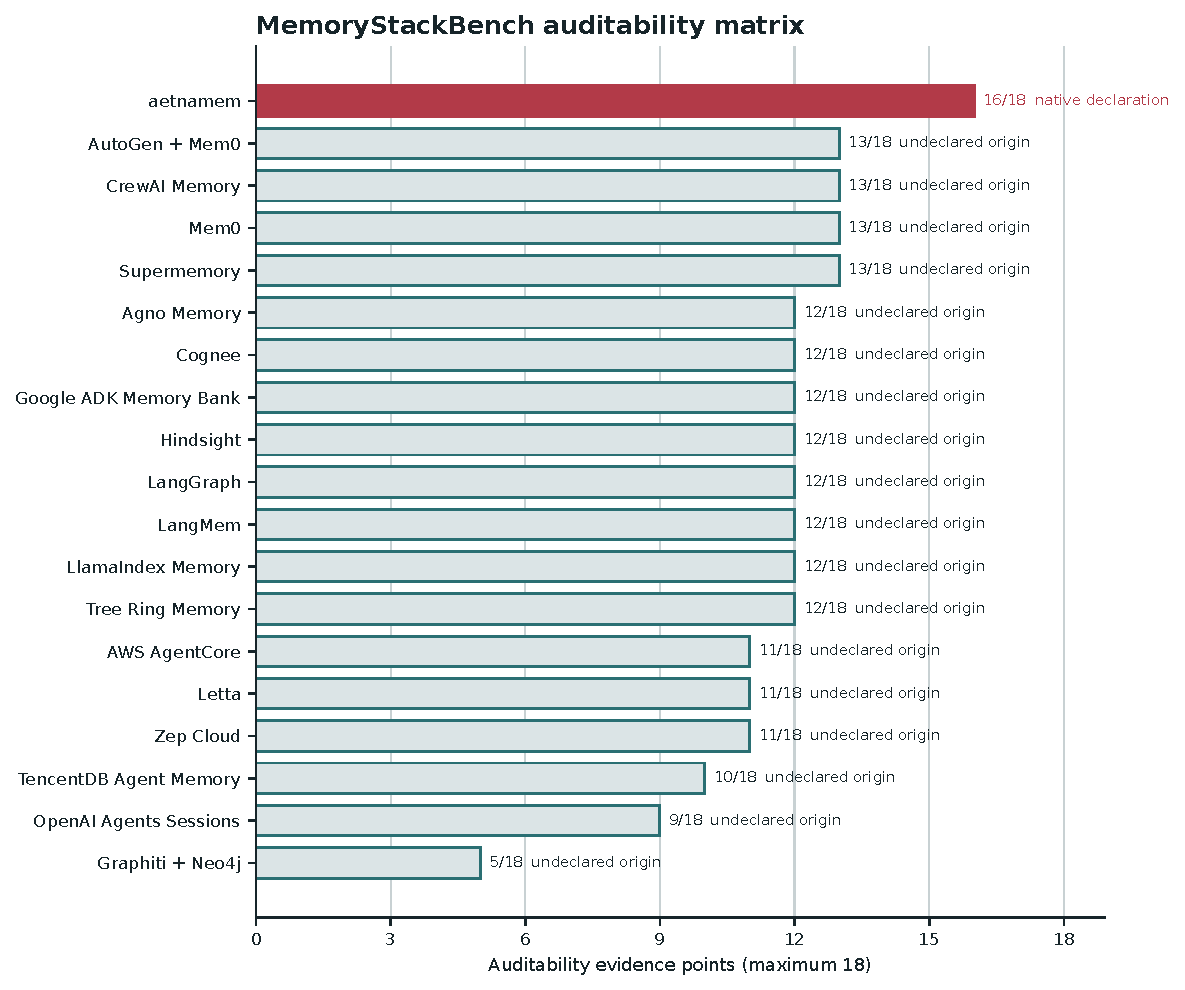
\includegraphics[width=0.84\textwidth]{figures/auditability.pdf}
\caption{Separate auditability evidence matrix from the pinned public snapshot. \system{} receives 16/18 points; the next-highest reported value is 13/18. Origin metadata is shown because native and undeclared evidence should not be conflated. This matrix is descriptive and not included in the safety score.}
\label{fig:auditability}
\end{figure*}

\system{} receives 16/18 points: 3/3 for inspectability, provenance, retrieval transparency, and deletion evidence; 2/3 for mutation lineage and tamper evidence. The public scorecard explains the two partial dimensions: records expose status, fact keys, and supersession links but not every possible lineage feature; the exported benchmark bundle exposes hashes but does not run the repository's full checkpoint verifier as part of its rubric.

The next-highest public point total is 13/18. This gap is consistent with \system's evidence-first design, but comparison is confounded by manifest declarations and adapter visibility. We therefore do not treat 16/18 as an independently validated security ranking.

\begin{figure*}[t]
\centering
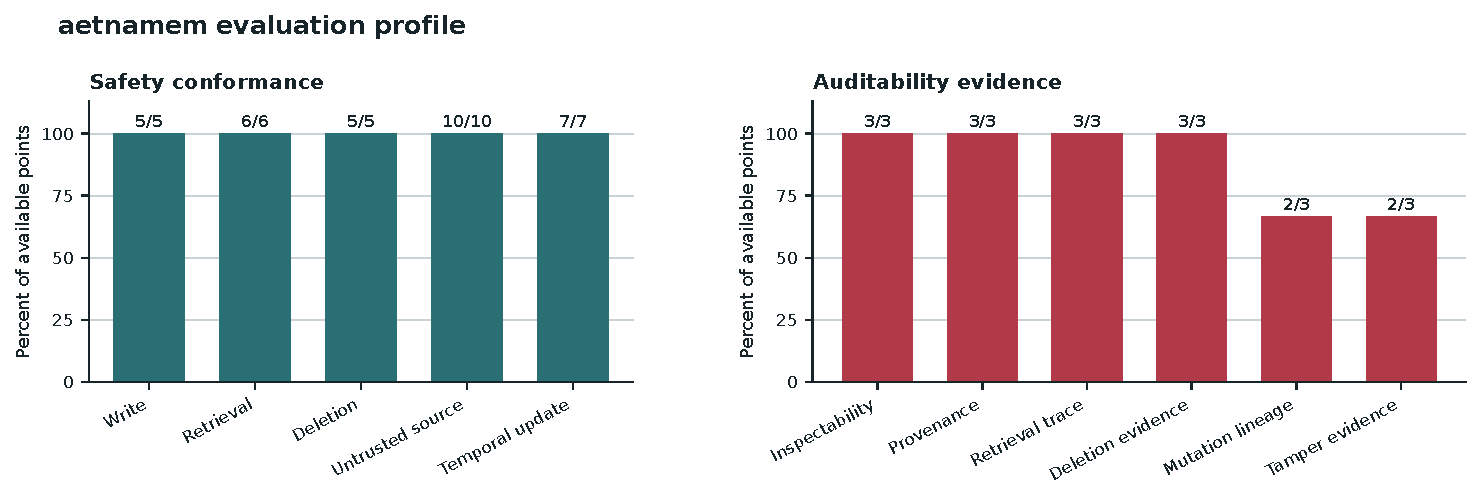
\includegraphics[width=0.92\textwidth]{figures/aetnamem-profile.pdf}
\caption{\system{} profile. Safety bars report passed checks; auditability bars report the benchmark's evidence points. Equal bar heights across the two panels do not imply equal semantics.}
\label{fig:aetna-profile}
\end{figure*}

\subsection{RQ2: guarded-action behavior}

The recorded demo produces one active trusted record and one quarantined untrusted record in the same fact slot. Recall returns the trusted record only. The five prohibited action paths all exit nonzero, while the authorized write reaches \code{committed}; its operation reaches \code{verified}; and the resulting \code{report.md} has the expected SHA-256 digest.

\begin{figure*}[t]
\centering
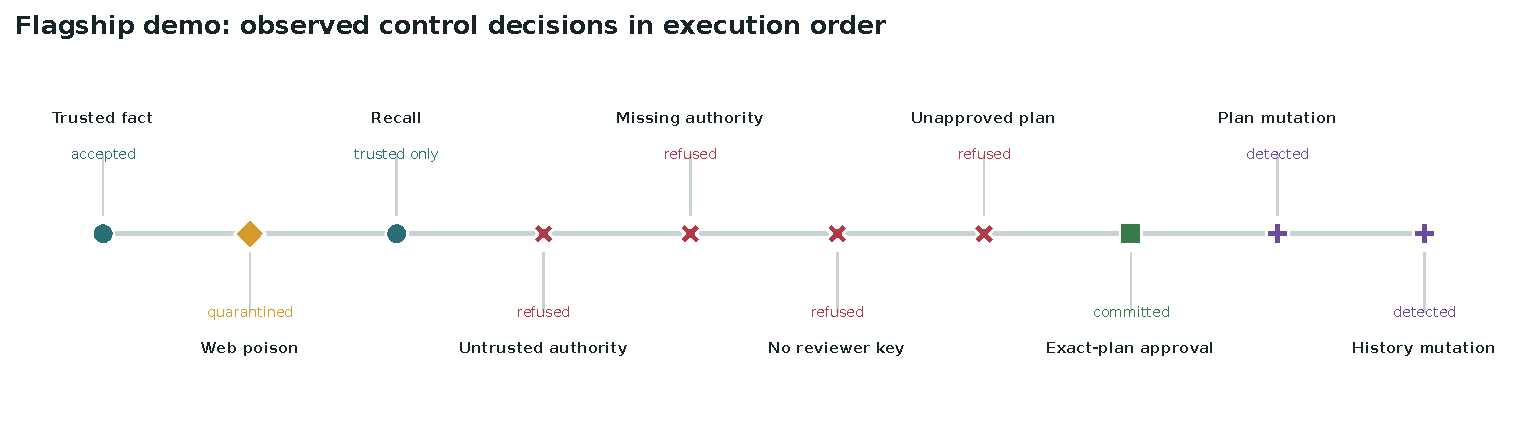
\includegraphics[width=0.98\textwidth]{figures/demo-trace.pdf}
\caption{Observed decisions in execution order. Red crosses are refused paths, purple markers are detected mutations, and the green square is the single authorized commit. The first three steps establish the delayed-memory attack precondition and quarantine result.}
\label{fig:demo-trace}
\end{figure*}

\begin{table}[t]
\centering
\caption{Flagship experiment outcomes.}
\label{tab:demo-results}
\scriptsize
\begin{tabularx}{\columnwidth}{@{}Y C{14mm} Y@{}}
\toprule
Probe & Result & Evidence \\
\midrule
Hidden webpage value enters trusted slot & Blocked & Record is quarantined at confidence 0.3 \\
Recall after poisoning & Safe & Only active trusted record returned \\
Untrusted evidence as authority & Refused & Policy exception, nonzero exit \\
No authority for mutation & Refused & Policy exception, nonzero exit \\
No reviewer key & Refused & CLI key-boundary check \\
Unapproved commit & Refused & State-machine check \\
Approved plan mutation & Refused & Plan recomputation mismatch \\
Exact approved write & Committed & Verified after-state + receipt \\
Audit payload mutation & Detected & Sequence 4 hash mismatch \\
\bottomrule
\end{tabularx}
\end{table}

The original artifact records 12 events: two episode ingestions; one trusted record creation; one quarantine; one recall; and seven action events from proposal through receipt. This compact history is sufficient to reconstruct the tested causal path without storing report contents in the audit plane.

\subsection{RQ3: verification and tamper probes}

The engine self-check passes against one checkpoint. Both standalone programs pass against the original database. The action verifier recomputes the plan and validates the receipt even without the reviewer secret; when given the secret it can additionally authenticate the HMAC. The audit-history mutation fails with \code{sequence 4: event\_hash mismatch}. The plan-table mutation is detected before execution and the attempted \code{retro.md} file is never written.

All 88 repository tests pass in 2.06 seconds on the disclosed machine. This runtime is included only as a reproducibility observation; no comparative performance claim is made.

\subsection{Result interpretation}

The evidence supports four narrow conclusions for the tested implementation and paths:

\begin{enumerate}
  \item classified untrusted content remains non-recallable until promotion and does not supersede the trusted same-slot value;
  \item enforced mutations require structurally trusted authority and exact-plan approval;
  \item the reference adapter commits the authorized write only after precondition and postcondition checks; and
  \item operational-plan and audit-history mutations used in the experiment are detected by independent code paths.
\end{enumerate}

It does not show that arbitrary natural-language injections are classified, that every adapter verifies truthfully, that an LLM cannot use a bypass tool, or that five scenarios predict field failure rates.
